\section{Exponential Distribution}

\subsection{Standard Exponential Distribution}

The PDF of the exponential distribution is

\begin{equation}
	p(x| \lambda) = \lambda \exp(-\lambda x)
	\label{eq:exponential_pdf}
\end{equation}

which can be written as

\begin{equation}
	p(x|\lambda) = \exp\left[-\lambda x + \log\lambda\right]
	\label{eq:exponential_exp_family}
\end{equation}

with $h(x) = 1$, $\phi(x)=x$, $w = -\lambda$ and $Z(\lambda) = -\log\lambda$

\subsubsection{Laplace Approximation of the Exponential Distribution}

\begin{align*}
\text{log-pdf: } &\left( \log \lambda - \lambda x\right) \\
\text{1st derivative: }& - \lambda \\
\text{2nd derivative: }& 0
\end{align*}
The Laplace Approximation is not defined since the second derivative is not positive. 

\subsection{Log-transformed Exponential Distribution}

We choose $X = \log(Y)$ and therefore $g(x) = \log(x)$, and $x(y) = g^{-1}(y) = \exp(y)$. Also, $\left\vert \frac{\partial x(y)}{\partial y}\right\vert = \exp(y)$. It follows that the new pdf is 

\begin{align}
	\mathcal{E}_{Y\log}(y; \lambda) &= \lambda \exp(-\lambda x(y)) \cdot \exp(y) \\ \nonumber
	&= \lambda \exp(-\lambda \exp(y) + y) \\
	&=  \exp\left[-\lambda \exp(y) + y + \log\lambda\right]
\end{align}

with $h(y) =1$, $\phi(x) = (y, \exp(y))$, $w = (1, -\lambda)$ and $Z(\lambda)=\log\lambda$

\subsubsection{Laplace Approximation of the log-transformed Exponential Distribution}

\begin{align*}
\text{log-pdf: } & -\lambda \exp(y) + y + \log\lambda \\
\text{1st derivative: }& \lambda -\exp(y) + 1 \\
\text{mode: } & y = \log(1/\lambda) \\
\text{2nd derivative: }& -\lambda\exp(y)\\
\text{insert mode: }& -\lambda\exp(1/\lambda) = -1\\
\text{invert \& times -1: }&\sigma^2 = 1
\end{align*}

Therefore the Laplace approximation in the transformed basis is given by $\mathcal{N}(y, \log(1/\lambda), 1)$. 

\subsection{The Bridge for the log-transformed Exponential Distribution}

We have already found $\mu$ and $\sigma$. The inverse transformation is easily found through the mode $\mu = \log(1/\lambda) \Leftrightarrow \lambda = 1/\exp(\mu)$. In summary:

\begin{align}
	\mu &= \log(1/\lambda) \\
	\sigma &= 1 \\
	\lambda &= 1/\exp(\mu)
\end{align}

\begin{figure}
	\centering
	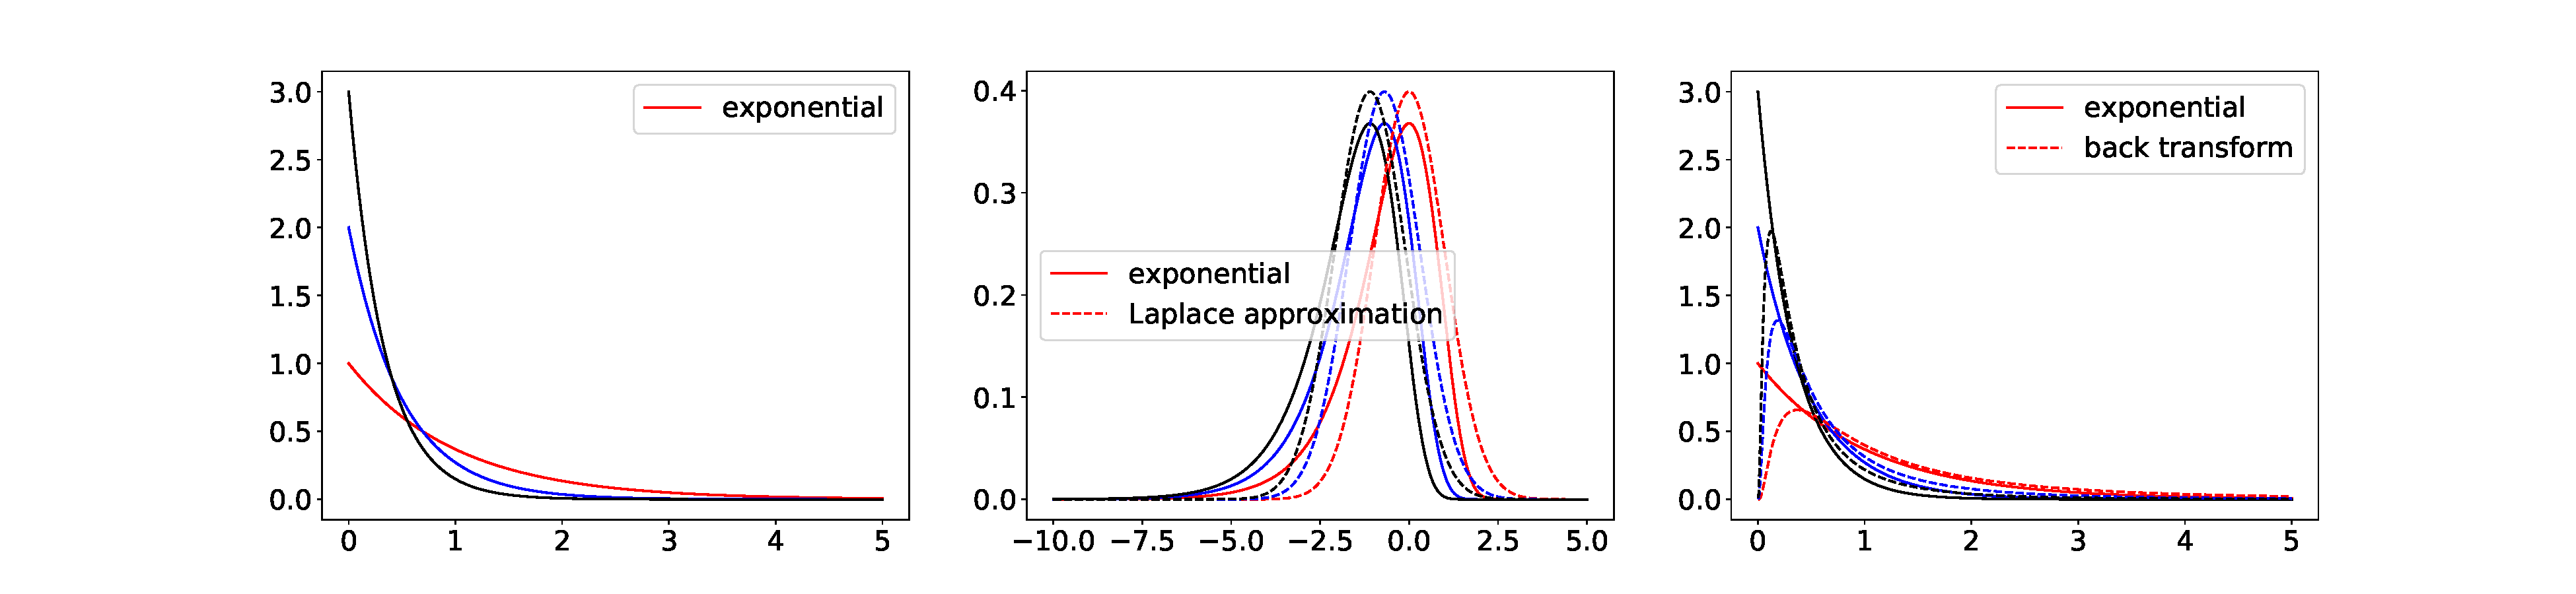
\includegraphics[width=\textwidth]{figures/exponential_playground.pdf}
	\caption{exponential comparison}
	\label{fig:exponential_comparison}
\end{figure}

\subsection{Sqrt-transformed Exponential Distribution}

We choose $X = \sqrt{Y}$ and therefore $g(x) = \sqrt{x}$, and $x(y) = g^{-1}(y) = y^2$. Also, $\left\vert \frac{\partial x(y)}{\partial y}\right\vert = 2y$. It follows that the new pdf is 

\begin{align}
\mathcal{E}_{Ysqrt}(y; \lambda) &= \lambda \exp(-\lambda y^2) \cdot 2y \\ \nonumber
&= 2 \cdot \exp\left[\log(y)-\lambda y^2 + \log\lambda\right] \\
\end{align}

with $h(y)=2$, $\phi(y) = (\log(y), y^2))$, $w = (1, -\lambda)$ and $Z(\lambda)=\log\lambda$

\subsubsection{Laplace Approximation of the sqrt-transformed Exponential Distribution}

\begin{align*}
\text{log-pdf: } & \log(2y)-\lambda y^2 + \log\lambda \\
\text{1st derivative: }& \frac{1}{y} - 2\lambda y \\
\text{mode: } & y = \sqrt{\frac{1}{2\lambda}}\\
\text{2nd derivative: }& -\frac{1}{y^2} - 2\lambda\\
\text{insert mode: }& -\frac{1}{\frac{1}{2\lambda}} - 2\lambda = -4\lambda\\
\text{invert \& times -1: }&\sigma^2 = \frac{1}{4\lambda}
\end{align*}

\subsection{The Bridge for the sqrt-transformed Exponential Distribution}

\begin{align}
	\mu &= \sqrt{\frac{1}{2\lambda}} \\
	\sigma^2 &= \frac{1}{4\lambda} \\
	\lambda &= \frac{1}{2\mu^2}
\end{align}